\begin{figure}[!htbp]
\begin{center}

\begin{minipage}[t]{0.5\linewidth}

% \begin{minipage}[b]{\linewidth}
% \begin{center}

% \begin{minipage}[t]{0.18\linewidth}
% \centering
% \vspace{0pt} % for alignment
% \adjincludegraphics[width=\textwidth, trim={{.0\width} {.77\width} {.79\width} {.02\width}}, clip]{img/lifecycle/burst-paint/seed=1034+title=directional_channel_grayscale_viz+treat=resource-wave__channelsense-yes__nlev-two+update=1048648+_data_hathash_hash=ca8ad21d3b30b939+_script_fullcat_hash=602c0d0c070e9202+_source_hash=53a2252-clean+ext=}
% \footnotesize Update 0
% \end{minipage}
% \begin{minipage}[t]{0.18\linewidth}
% \centering
% \vspace{0pt} % for alignment
% \adjincludegraphics[width=\textwidth, trim={{.0\width} {.77\width} {.79\width} {.02\width}}, clip]{img/lifecycle/burst-paint/seed=1034+title=directional_channel_grayscale_viz+treat=resource-wave__channelsense-yes__nlev-two+update=1048744+_data_hathash_hash=ca8ad21d3b30b939+_script_fullcat_hash=602c0d0c070e9202+_source_hash=53a2252-clean+ext=}
% \footnotesize 96
% \end{minipage}
% \begin{minipage}[t]{0.18\linewidth}
% \centering
% \vspace{0pt} % for alignment
% \adjincludegraphics[width=\textwidth, trim={{.0\width} {.77\width} {.79\width} {.02\width}}, clip]{img/lifecycle/burst-paint/seed=1034+title=directional_channel_grayscale_viz+treat=resource-wave__channelsense-yes__nlev-two+update=1048840+_data_hathash_hash=ca8ad21d3b30b939+_script_fullcat_hash=602c0d0c070e9202+_source_hash=53a2252-clean+ext=}
% \footnotesize 192
% \end{minipage}
% \begin{minipage}[t]{0.18\linewidth}
% \centering
% \vspace{0pt} % for alignment
% \adjincludegraphics[width=\textwidth, trim={{.0\width} {.77\width} {.79\width} {.02\width}}, clip]{img/lifecycle/burst-paint/seed=1034+title=directional_channel_grayscale_viz+treat=resource-wave__channelsense-yes__nlev-two+update=1048936+_data_hathash_hash=ca8ad21d3b30b939+_script_fullcat_hash=602c0d0c070e9202+_source_hash=53a2252-clean+ext=}
% \footnotesize 288
% \end{minipage}
% \begin{minipage}[t]{0.18\linewidth}
% \centering
% \vspace{0pt} % for alignment
% \adjincludegraphics[width=\textwidth, trim={{.0\width} {.77\width} {.79\width} {.02\width}}, clip]{img/lifecycle/burst-paint/seed=1034+title=directional_channel_grayscale_viz+treat=resource-wave__channelsense-yes__nlev-two+update=1049032+_data_hathash_hash=ca8ad21d3b30b939+_script_fullcat_hash=602c0d0c070e9202+_source_hash=53a2252-clean+ext=}
% \footnotesize 384
% \end{minipage}
% \caption{Wild type timelapse}
% \label{fig:wt_timelapse}
% \end{center}
% \end{minipage}

% \vspace{2ex}

\begin{minipage}[b]{\linewidth}
\begin{center}

\begin{minipage}[t]{0.30\linewidth}
\centering
\vspace{0pt} % for alignment
% adapted from https://tex.stackexchange.com/a/186476
\begin{tikzpicture}
\node[anchor=south west,inner sep=0] (image) at (0,0) { \adjincludegraphics[width=\linewidth, trim={{.25\width} {.20\width} {.5\width} {.55\width}}, clip]{img/knockout/interior_propagule/wildtype/retouched3_seed=1+title=directional_regulator_viz+treat=resource-wave__channelsense-yes__nlev-two+update=8188+_data_hathash_hash=8b493febd79aad1f+_script_fullcat_hash=90718bb0c6ec4dbd+_source_hash=53a2252-clean+ext=}
};
\begin{scope}[x={(image.south east)},y={(image.north west)}]
  \draw [ultra thick,-{stealth[scale=1.25]}, white] (0.35,0.59) -- ++(0.06,-0.06);
  \draw [ultra thick, -{stealth[scale=1.25]}, white] (0.01,0.39) -- ++(0.06,-0.06);
  \draw [ultra thick, -{stealth[scale=1.25]}, white] (0.68,0.39) -- ++(0.06,-0.06);
  \draw [ultra thick, -{stealth[scale=1.25]}, white] (0.62,0.32) -- ++(0.06,-0.06);
  \draw [-stealth, red] (0.35,0.59) -- ++(0.05,-0.05);
  \draw [-stealth, red] (0.01,0.39) -- ++(0.05,-0.05);
  \draw [-stealth, red] (0.68,0.39) -- ++(0.05,-0.05);
  \draw [-stealth, red] (0.62,0.32) -- ++(0.05,-0.05);
\end{scope}
\end{tikzpicture}
\footnotesize Wild type
\end{minipage}
\begin{minipage}[t]{0.30\linewidth}
\centering
\vspace{0pt} % for alignment
\adjincludegraphics[width=\linewidth, trim={{.5\width} {.5\width} {.25\width} {.25\width}}, clip]{img/knockout/interior_propagule/propaguleknockout/retouched2_seed=1+title=directional_regulator_viz+treat=resource-wave__channelsense-yes__nlev-two+update=8188+_data_hathash_hash=2b6711db47fb5887+_script_fullcat_hash=90718bb0c6ec4dbd+_source_hash=53a2252-clean+ext=}
\footnotesize Propagule knockout
\end{minipage}
\begin{minipage}[t]{0.30\linewidth}
\centering
\vspace{0pt} % for alignment
\adjincludegraphics[width=\linewidth, trim={{.5\width} {.5\width} {.25\width} {.25\width}}, clip]{img/knockout/interior_propagule/regulationknockout/retouched_seed=1+title=directional_regulator_viz+treat=resource-wave__channelsense-yes__nlev-two+update=8188+_data_hathash_hash=11ab5cdd47ed18c7+_script_fullcat_hash=90718bb0c6ec4dbd+_source_hash=53a2252-clean+ext=}
\footnotesize Regulation knockout
\end{minipage}

{\textbf{(A)} Regulation visualizations}
% \label{fig:regulation_visualizations}

\end{center}
\end{minipage}

\begin{minipage}[t]{\linewidth}
\centering
\vspace{0pt} % for alignment
\begin{minipage}[b]{\linewidth}
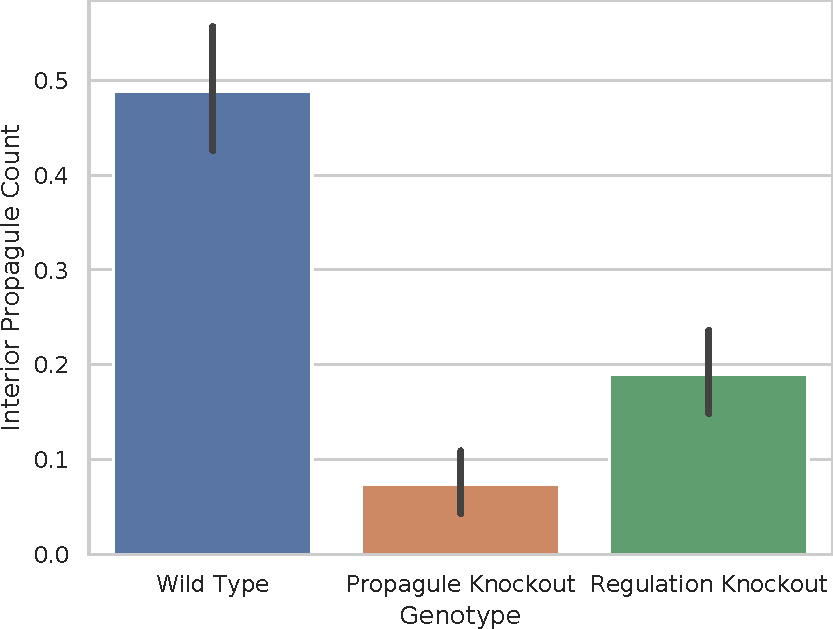
\includegraphics[width=\linewidth]{img/knockout/interior_propagule/title=interior_propagules+_data_hathash_hash=bb0fa6254f1b7398+_script_fullcat_hash=f738b363bea8c98a+_source_hash=53a2252-clean+ext=}
{\textbf{(B)} Interior propagule rate by genotype}
% \label{fig:interior_propagule_rate}
\end{minipage}
\end{minipage}%
\hspace*{\fill}

\end{minipage}

\caption{
Analysis of a wild type strain exhibiting a ``burst'' lifecycle evolved under the ``Nested-Wave'' treatment exhibiting interior propagule generation.
% Figure \ref{fig:wt_timelapse} traces the wild type life history.
% L1 hereditary groups are by differentiated by grayscale tone and separated by solid black borders.
% L0 hereditary groups are by separated by gray borders.
% In each example, the focal parent L1 hereditary group is colored purple and the focal offspring group orange.
Subfigure \textbf{(A)} compares gene regulation between analyzed strains.
Group layouts are overlaid via borders between cells.
Black borders divide L1 groups and white borders divide L0 groups.
Borders between L1 groups are underlined in red for greater visibility.
Within these group layouts, regulation state for each cell's four directional SignalGP instances is color coded using a PCA mapping from regulatory state to three-dimensional RGB coordinates.
(The PCA mapping is calculated uniquely for each L1 hereditary group.)
Within a L1 hereditary group, color similarity among tile quarters indicates that the corresponding SignalGP instances exhibit similar regulatory state.
In the case of identical regulatory state (here, due to the absence of genetic regulation in a knockout strain) this color coding appears gray.
Wild type interior propagules are annotated with red arrows.
Subfigure \textbf{(B)} compares the mean number of interior propagules observed per L1 hereditary group.
Error bars indicate 95\% confidence.
View an animation of wild type gene regulation at \url{https://hopth.ru/t}.
View the wild type strain in a live in-browser simulation at \url{https://hopth.ru/g}.
}
\label{fig:ko-interior_propagule}
\end{center}
\end{figure}
